
%(BEGIN_QUESTION)
% Copyright 2007, Tony R. Kuphaldt, released under the Creative Commons Attribution License (v 1.0)
% This means you may do almost anything with this work of mine, so long as you give me proper credit

Often, the phrase {\it quarter-amplitude damping} (sometimes called {\it quarter-wave} damping) is used to describe good process response to a disturbance or setpoint change (perturbation).  What does this phrase mean?  Sketch the response of a process to a setpoint change (continue the PV plot), where the controller has been tuned for quarter-wave damping:

$$\includegraphics[width=15.5cm]{i01668x01.eps}$$

\underbar{file i01668}
%(END_QUESTION)





%(BEGIN_ANSWER)

The controller output graph shown here is {\it qualitative} only.  Although drawn to scale (i.e. all changes in the output are properly scaled relative to each other), the scale itself is arbitrary and therefore may not match the scale of your sketch:

$$\includegraphics[width=15.5cm]{i01668x02.eps}$$

{\it Quarter-amplitude damping} means that the oscillations of process variable (PV) following a disturbance will decay, with each successive peak being 1/4 the amplitude of the one before.  This is considered by many to be a ``baseline'' standard for loop tuning, and not necessarily optimum.  For many types of processes, oscillations of this nature would be unacceptable.

%(END_ANSWER)





%(BEGIN_NOTES)


%INDEX% Control, PID tuning: quarter-wave damping controller response

%(END_NOTES)


